\documentclass[
    oneside, % no mirrored margin for twosided book
    % draft, % no figure, no listings, draw Bold where box overflow (debug)
    12pt % fontsize
]{article}

% !TeX root = ../main.tex
\usepackage[russian]{babel}
\usepackage{luacode}

\usepackage{fontspec}
\setmainfont{CMU Serif} % You can change this to your desired font
\setmonofont{DejaVu Sans Mono} 

\usepackage{amsmath} % math
\usepackage{amssymb}
\usepackage{mathtools}

\usepackage{numerica} % math calc


\usepackage[
    cachedir=output/_minted
]{minted}
\setminted{
    linenos, % line numbering
    breaklines, % wrap line if not fit
    frame=single % line box around
}

\usepackage{graphicx}

\usepackage{indentfirst} % красная строка

\usepackage{vmargin} % page size and margin
\setpapersize{A4}
\setmarginsrb{2cm}{1.5cm}{1cm}{1.5cm}{0pt}{0mm}{0pt}{13mm}
\directlua{
    dofile("lua/define_latex.lua")
    dofile("lua/util.lua")
} 


\newcommand{\thegroup}{1445}
\newcommand{\workyear}{\the\year}

\newcommand{\underoverline}[3][5cm]{
    \begin{minipage}{#1}
        \centering \vspace{1em}
        #2 \\
        \vspace{-0.9em}
        \rule{\textwidth}{0.5pt} \\
        \vspace{-0.3em}
        \footnotesize #3
    \end{minipage}
}

% Params
% #1 - Номер кафедры
% #2 - Должность, уч степень, звание преподавателя 
% #3 - ФИО преподавателя
% #4 - Тип работы и номер (Лабораторная работа №1)
% #5 - Название работы
% #6 - название курса
% #7 - ФИО студента(ов) (через запятую)
\newcommand{\maketitleguap}{
    \begin{titlepage}
        \centerline{ГУАП}
        \vfill
        \centerline{Кафедра №\getDepartmentNum}
        \vfill
        \leftline{ОТЧЕТ}
        \leftline{ЗАЩИЩЕН С ОЦЕНКОЙ}
        \vspace{0.7em}
        \leftline{ПРЕПОДАВАТЕЛЬ}
        \vspace{1em}
        
        
        \underoverline[6cm]{\getTeacherDegree\vphantom{AА}}{должность, уч. степень, звание}
        \underoverline[4cm]{\vphantom{AА}}{подпись, дата}
        \underoverline[6cm]{\getTeacherName}{фамилия, инициалы}
        
        \vfill
        \centerline{\large \uppercase{\getWorkType}}
        \vfill
        \centerline{\large \uppercase{\getWorkName}}
        \vfill
        \centerline{по курсу:}
        \vspace{1em}
        \centerline{\large \uppercase{\getCourseName}}
        \vfill
        \vfill
        \begin{tabular}{lccc}
            \multicolumn{2}{l}{РАБОТУ \ifmany{\getWorkAuthor}{ВЫПОЛНИЛи}{ВЫПОЛНИЛ}} & & \\
            
            \ifmany{\getWorkAuthor}{СТУДЕНТы}{СТУДЕНТ} гр № &
            \underoverline[1.1cm]{\getWorkAuthorGroup\vphantom{1234}}{\phantom{1234}}
            \printSignName{\getWorkAuthor}
            % &
            % &
            % \underline{\hspace{4cm}} &
            % \underline{\hspace{1.5cm}\getWorkAuthor\hspace{1.5cm}} \\
            
            &
            &
            {\footnotesize подпись, дата} &
            {\footnotesize фамилия, инициалы}
        \end{tabular}
        
        \vfill
        \centerline{Санкт-Петербург \workyear}
    \end{titlepage}
    \addtocounter{page}{1} % increment page number
}



\begin{document}


\graphicspath{{img/}}

\captionsetup[table]{
    format=plain,
    font=small, labelformat=simple, labelsep=colon, % none colon period space quad newline endash
    justification=raggedright, 
    singlelinecheck=false, % margin one line too
    skip=5pt,
    position=above,
} % Customize table captions
% -------------------- BEGIN DOCUMENT --------------------

\departmentNum{14}
\teacherDegree{Boy nextdoor}
\teacherName{Letter man}
\workType{Лабораторная работа №42}
\workName{Fisting anal}
\courseName{Fuck you letterman}

\workAuthorGroup{1445}
\workAuthor{Boss of the gym, Slave}

\maketitleguap


\section{Задание 1.7.}

Из круга радиуса $R$ вырезали квадрат со стороной $a$. Какова площадь оставшейся фигуры?


\section{Формализация.}

Формулы площади фигур: $ S_{\text{круг}} = \pi R^2 $ и $ S_{\text{кв}} = a^2 $.

Площадь фигуры, полученная вычитанием из круга квадрата: $ s = S_{\text{круг}} - S_{\text{кв}} = \pi R^2 - a^2  $.

Для программного решения задачи, объявим переменные \texttt{r}, \texttt{a}, \texttt{s} с типом \texttt{float},
затем сделаем ввод $R$ и $a$, используя функцию \texttt{scanf}, 
для красивого оформления, предварительно выведем имена переменных с помощью \texttt{printf}.

Далее по формуле подсчитаем ответ и запишем в перменную \texttt{s}.

В конце выведем ответ, используя \texttt{printf}.

\newcommand{\formula}[2]{
    % \eval[vv=]{$ \pi R^2 - a^2 $}[R=#1,a=#2] % formula = answer
    \eval{$ \pi R^2 - a^2 $}[R=#1,a=#2]
}

\section{Блок-схема.}

\begin{figure}[h] % 'h' means place the figure here
    \centering % Center the image
    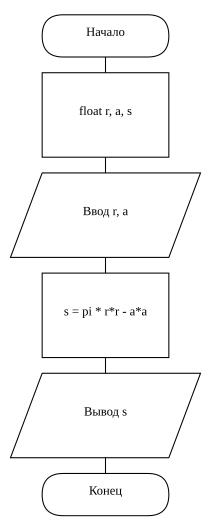
\includegraphics[height=15cm]{scheme} 
    \caption{Блок-схема.} % Caption for the image
    \label{fig:scheme} % Label for referencing the image
\end{figure}


\section{Программа.}

\inputminted{Lua}{lua/import.lua}

\section{Тестирование.}

\begin{table}[h]
    \caption{Тестирование.}
    \begin{tabular}{|l|cc|c|c|}
        \hline
        № & Ввод R & Ввод a & Расчет & Вывод программы \\
        \hline
        1 & 1   & 1   & \formula{1}{1}     & 2.141593     \\
        2 & 10  & 2   & \formula{10}{2}    & 310.159271  \\
        3 & 5   & 6   & \formula{5}{6}     & 42.539818   \\
        4 & 8   & 10  & \formula{8}{10}    & 101.061928  \\
        5 & 150 & 200 & \formula{150}{200} & 30685.833984\\
        \hline
    \end{tabular}
\end{table}

\section{Вывод.}

В первой лабораторной работе нужно было составить программу чтобы выполнить геометрический расчет. 
Блок схема составлена. Данные сошлись. Работа корректна.


\end{document}
